\section{Benchmark Results}
\label{cha:results}

In this section, we present and compare the findings from the data analysis across each targeted datastore. Throughout the benchmarking sessions, no CPU performance issues were detected on the client-side (load generator), ensuring that client limitations did not impact latency measurements. Additionally, the error rate consistently remained at zero for all runs, indicating that every read request was successfully completed.

\begin{figure}[h]
	\begin{subfigure}{0.49\linewidth}
		\centering
		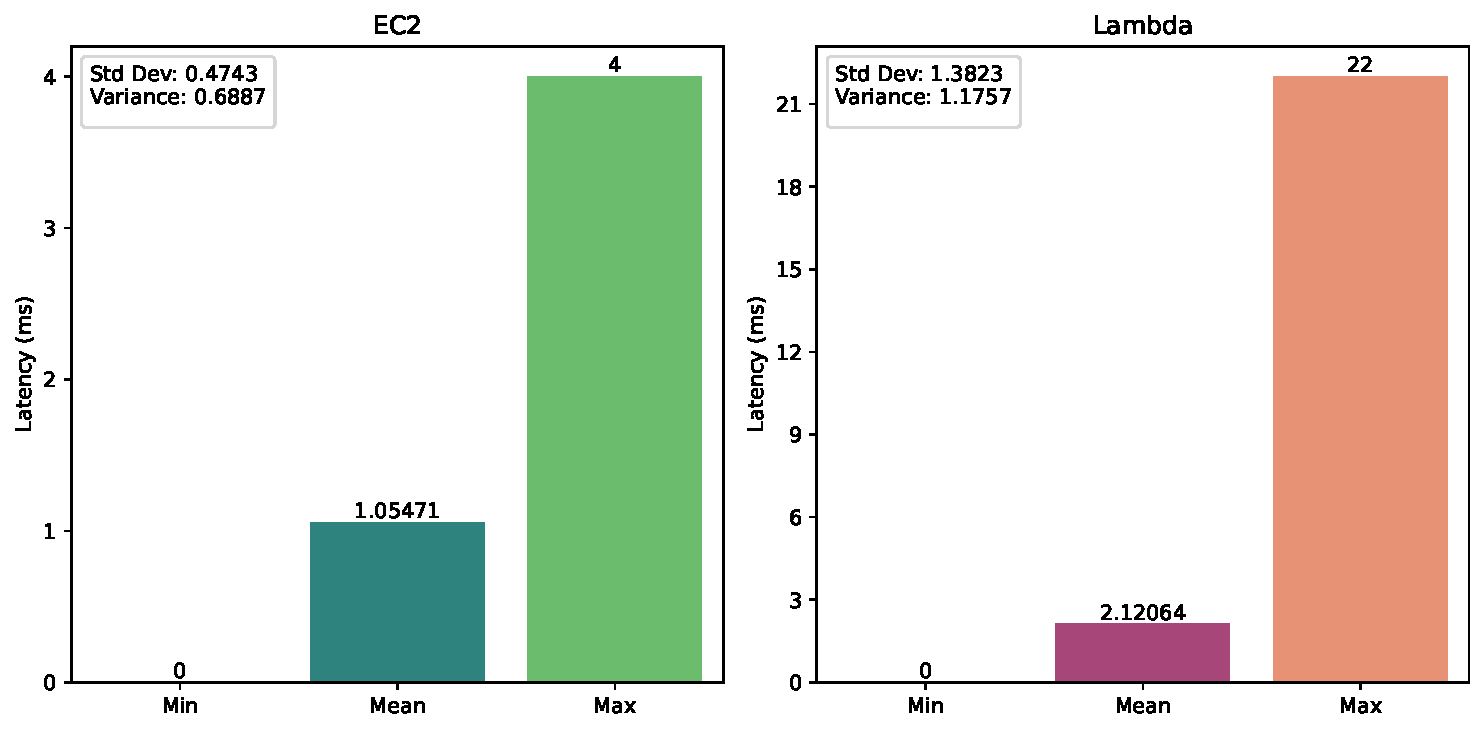
\includegraphics[width=\linewidth]{./fig/bar-rds-constant.pdf}
		\caption{Constant Load on RDS}
		\label{fig:bar_rds_const}
	\end{subfigure}
	\hfill
	\begin{subfigure}{0.49\linewidth}
		\centering
		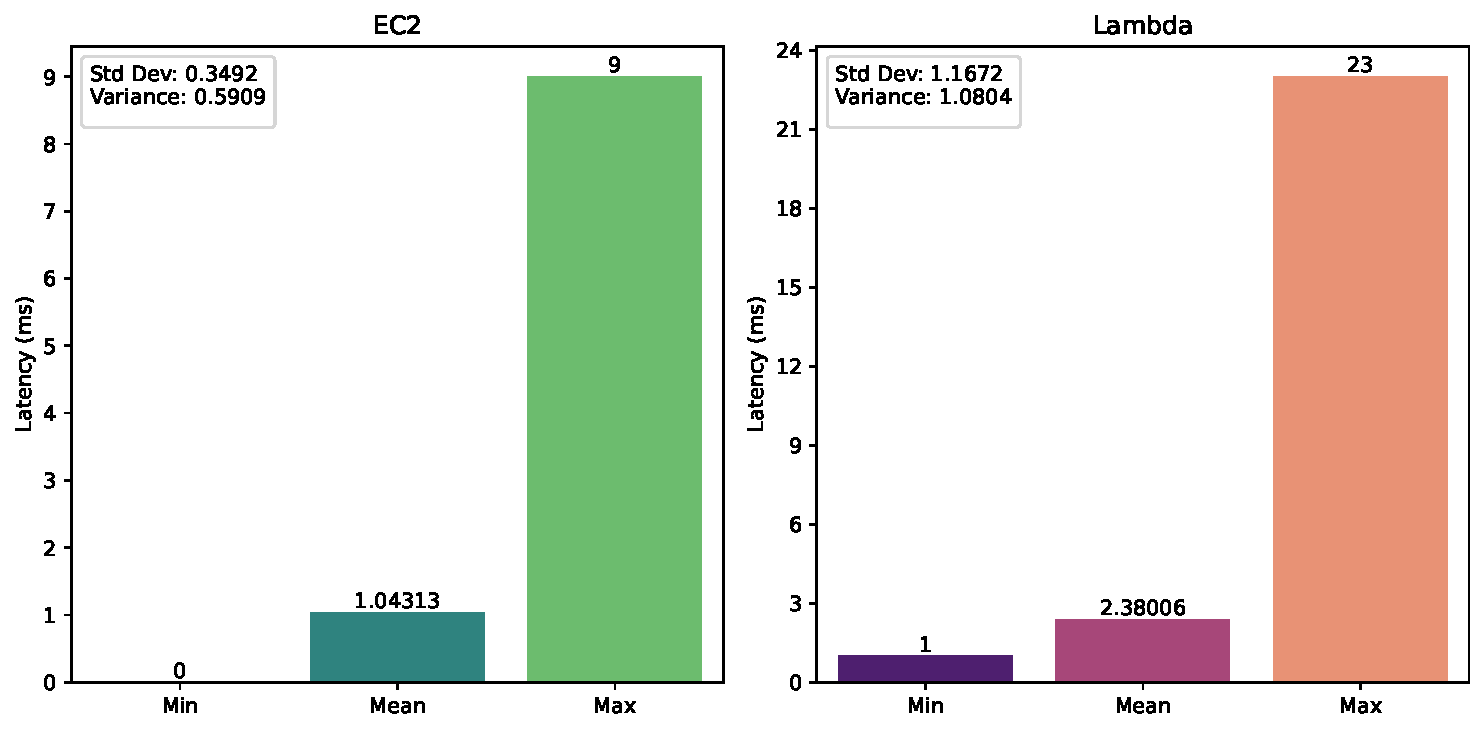
\includegraphics[width=\linewidth]{./fig/bar-rds-bursty.pdf}
		\caption{Bursty Load on RDS}
		\label{fig:bar_rds_bursty}
	\end{subfigure}
	\vfill
	\begin{subfigure}{0.49\linewidth}
		\centering
		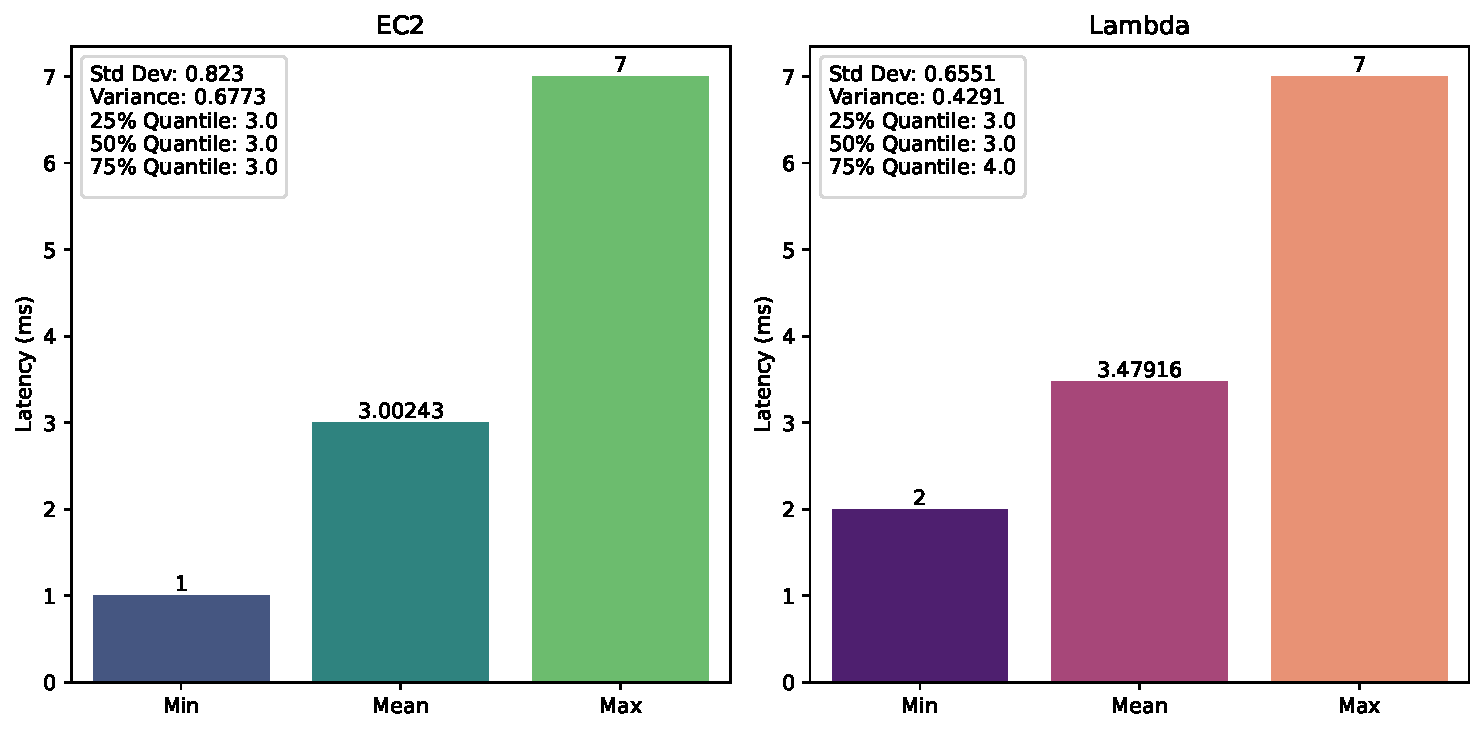
\includegraphics[width=\linewidth]{./fig/bar-dynamo-constant.pdf}
		\caption{Constant Load on DynamoDB}
		\label{fig:bar_ddb_const}
	\end{subfigure}
	\hfill
	\begin{subfigure}{0.49\linewidth}
		\centering
		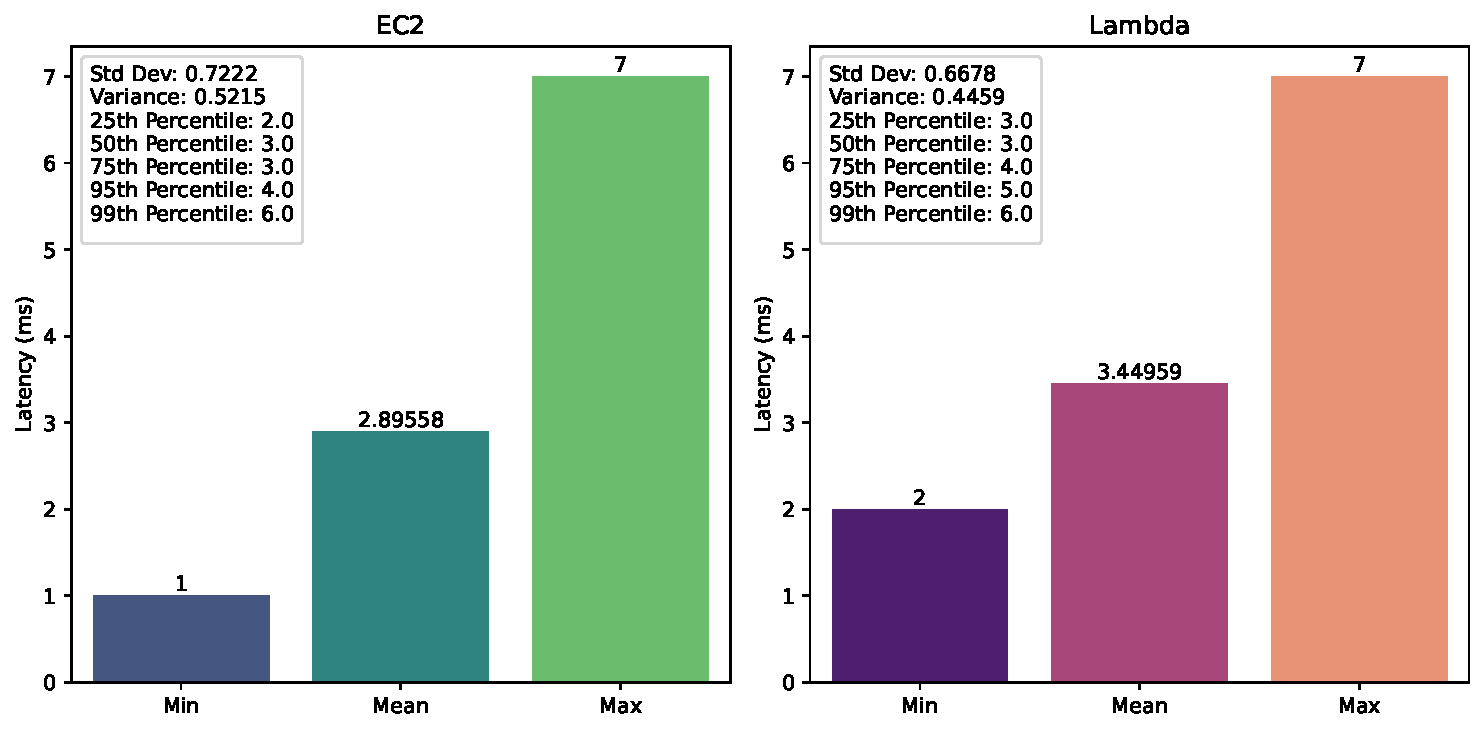
\includegraphics[width=\linewidth]{./fig/bar-dynamo-bursty.pdf}
		\caption{Bursty Load on DynamoDB}
		\label{fig:bar_ddb_bursty}
	\end{subfigure}
	\vfill
	\begin{subfigure}{0.49\linewidth}
		\centering
		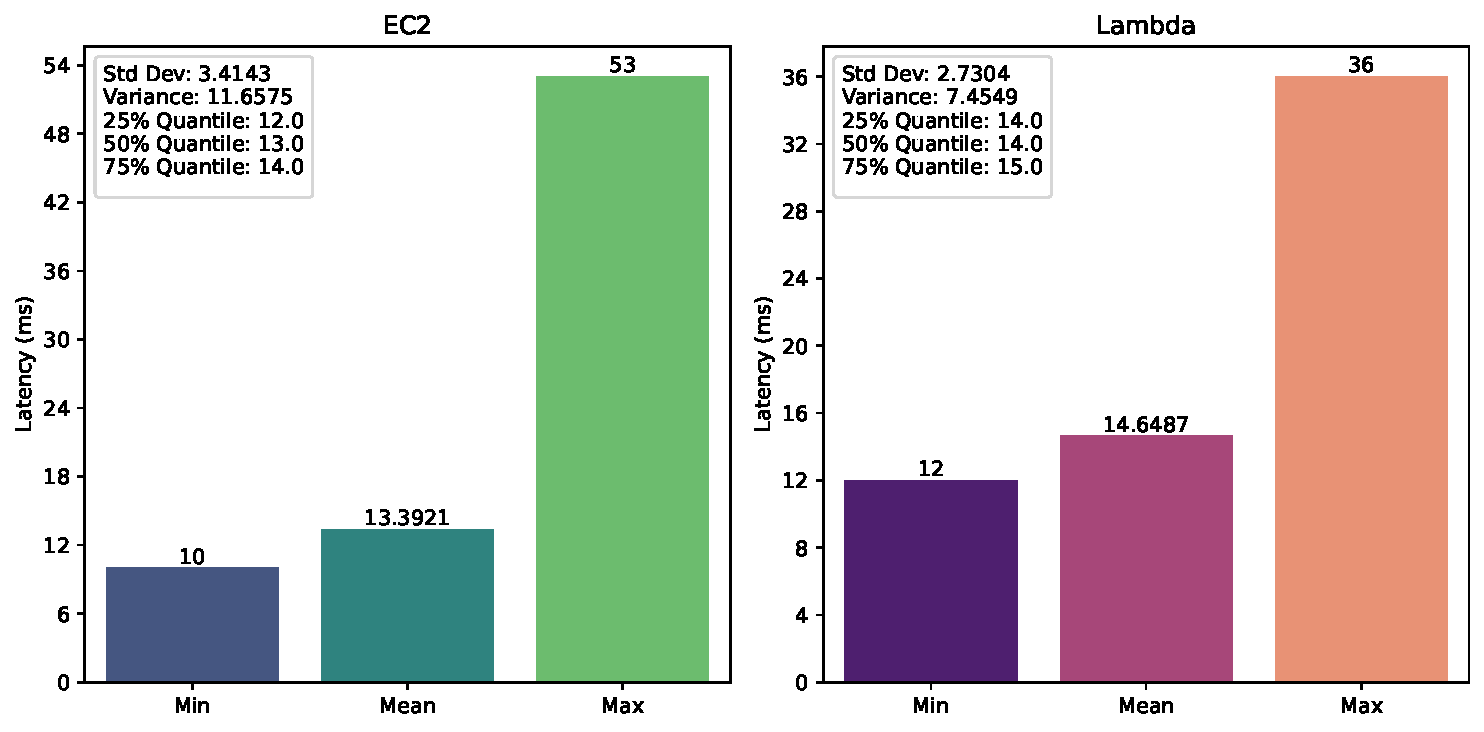
\includegraphics[width=\linewidth]{./fig/bar-s3-constant.pdf}
		\caption{Constant Load on S3}
		\label{fig:bar_s3_const}
	\end{subfigure}
	\hfill
	\begin{subfigure}{0.49\linewidth}
		\centering
		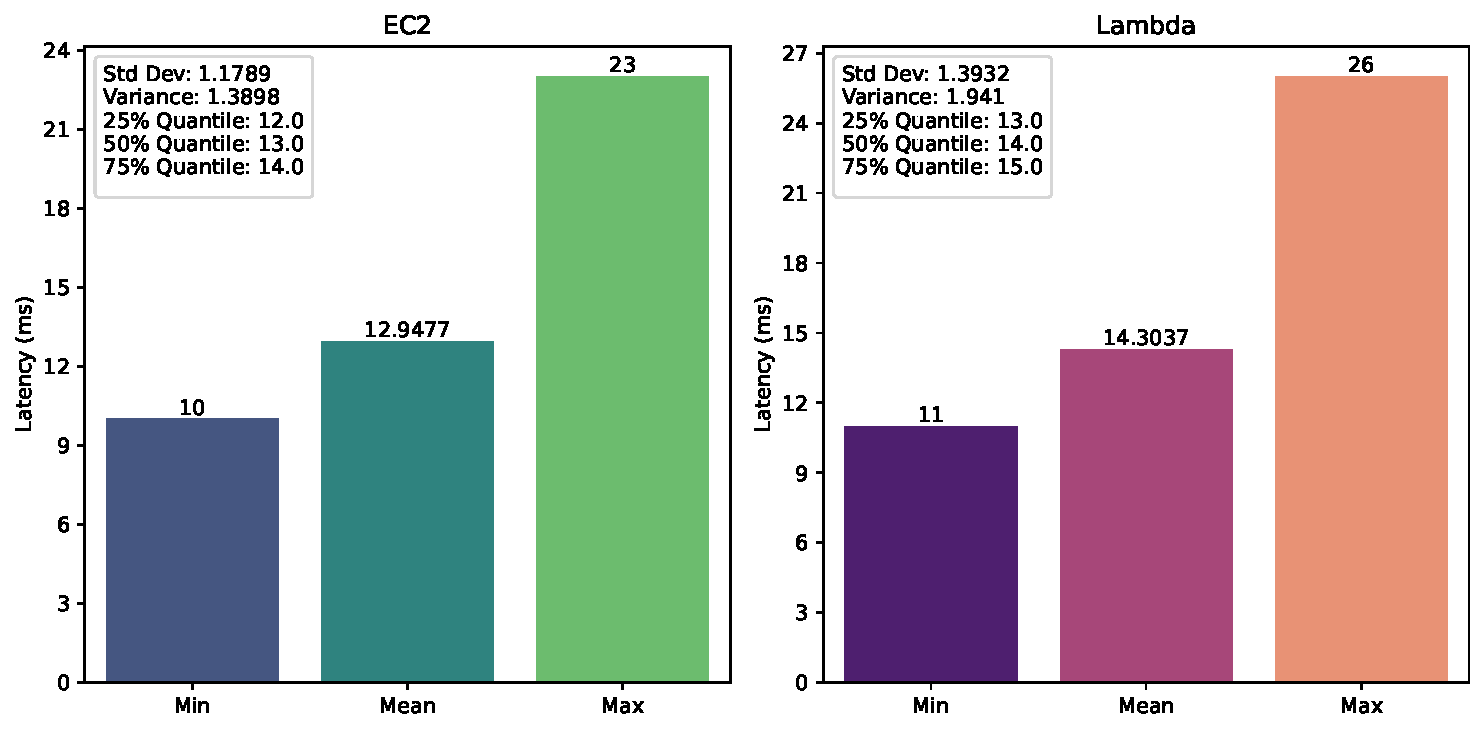
\includegraphics[width=\linewidth]{./fig/bar-s3-bursty.pdf}
		\caption{Bursty Load on S3}
		\label{fig:bar_s3_bursty}
	\end{subfigure}
	\caption{Aggregation of Latency Metric}
	\label{fig:bar-plots}
\end{figure}

\begin{figure}[h]
	\begin{subfigure}{0.49\linewidth}
		\centering
		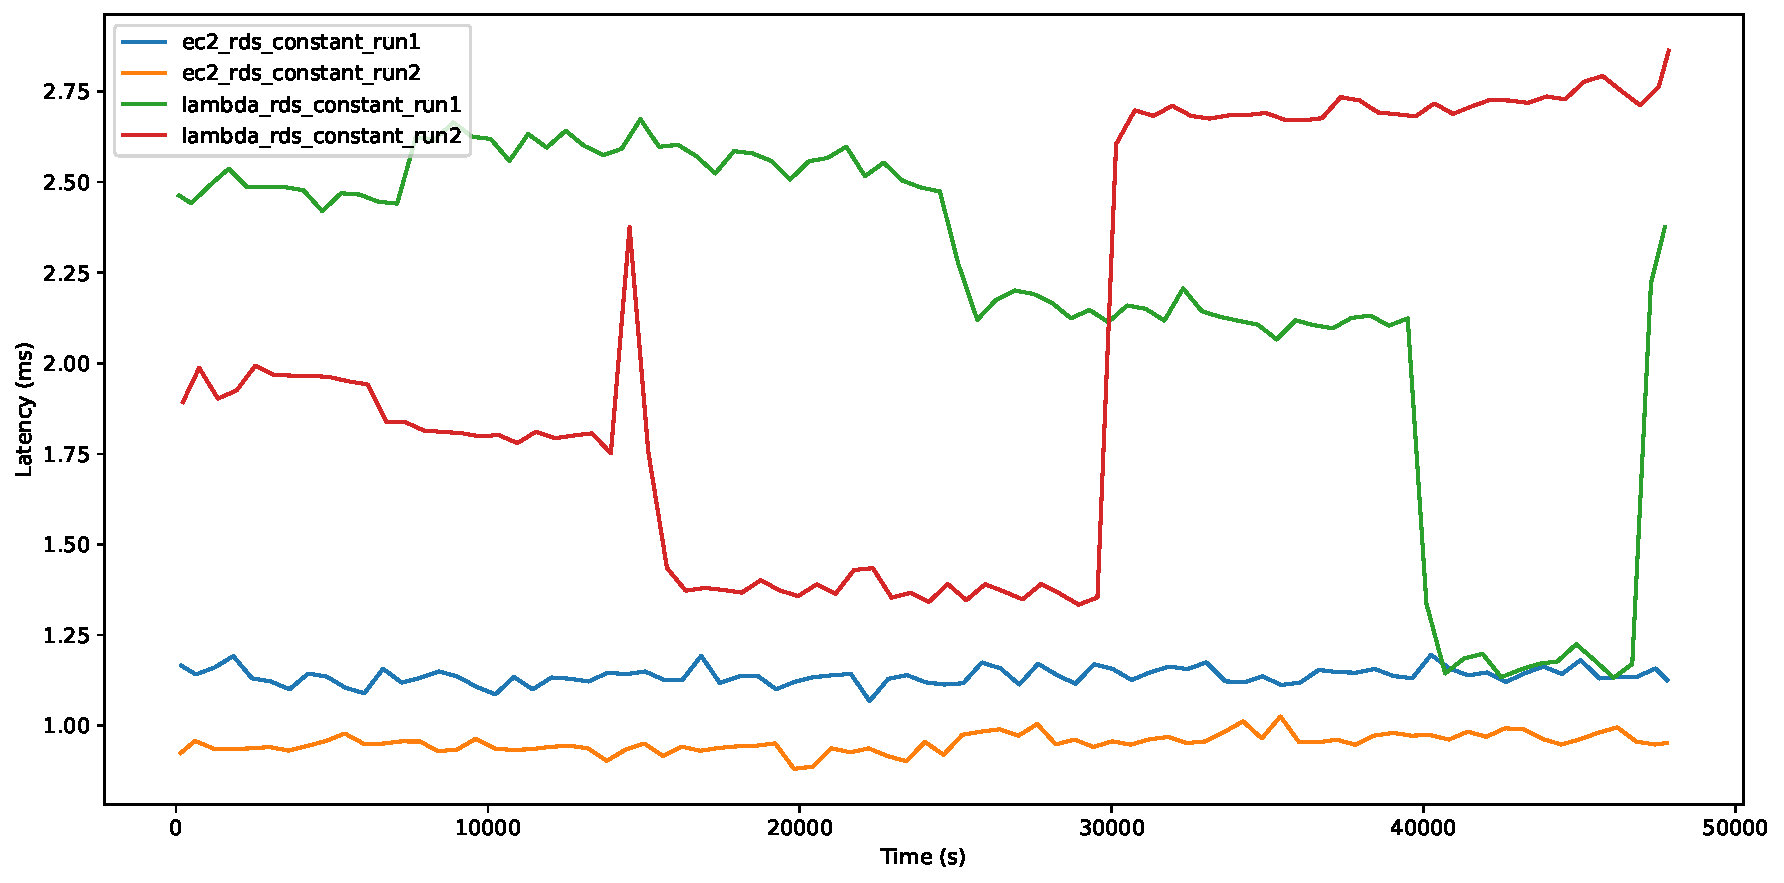
\includegraphics[width=\linewidth]{./fig/ts-rds-constant.pdf}
		\caption{Constant Load on RDS}
		\label{fig:ts_rds_const}
	\end{subfigure}
	\hfill
	\begin{subfigure}{0.49\linewidth}
		\centering
		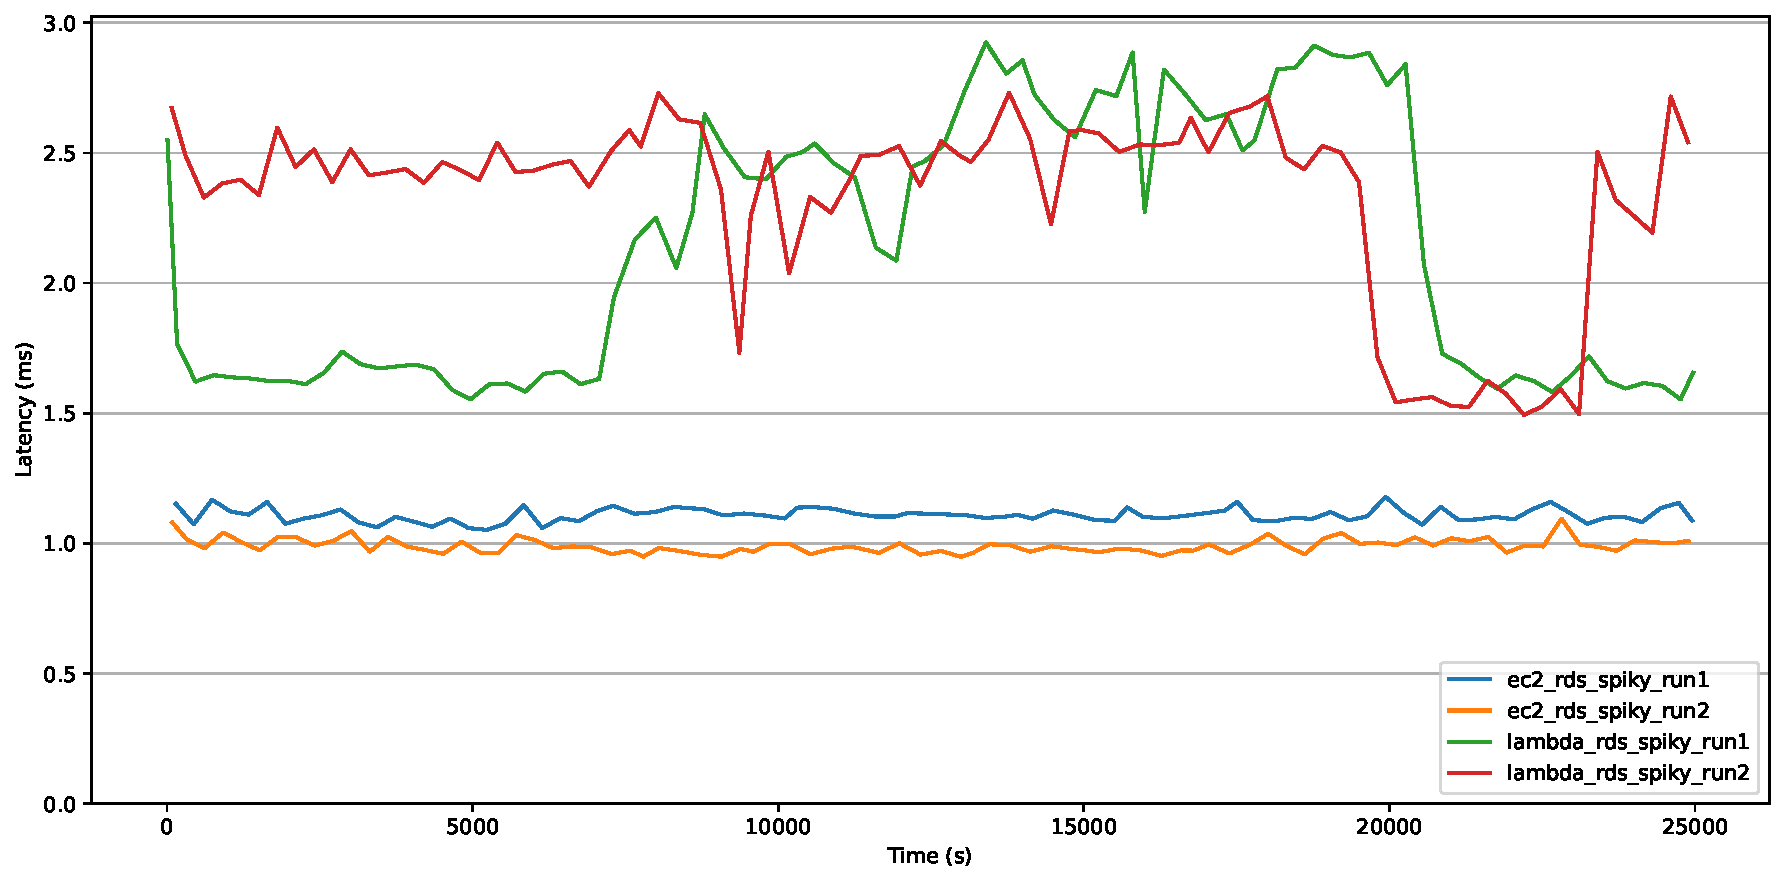
\includegraphics[width=\linewidth]{./fig/ts-rds-bursty.pdf}
		\caption{Bursty Load on RDS}
		\label{fig:ts_rds_bursty}
	\end{subfigure}
	\vfill
	\begin{subfigure}{0.49\linewidth}
		\centering
		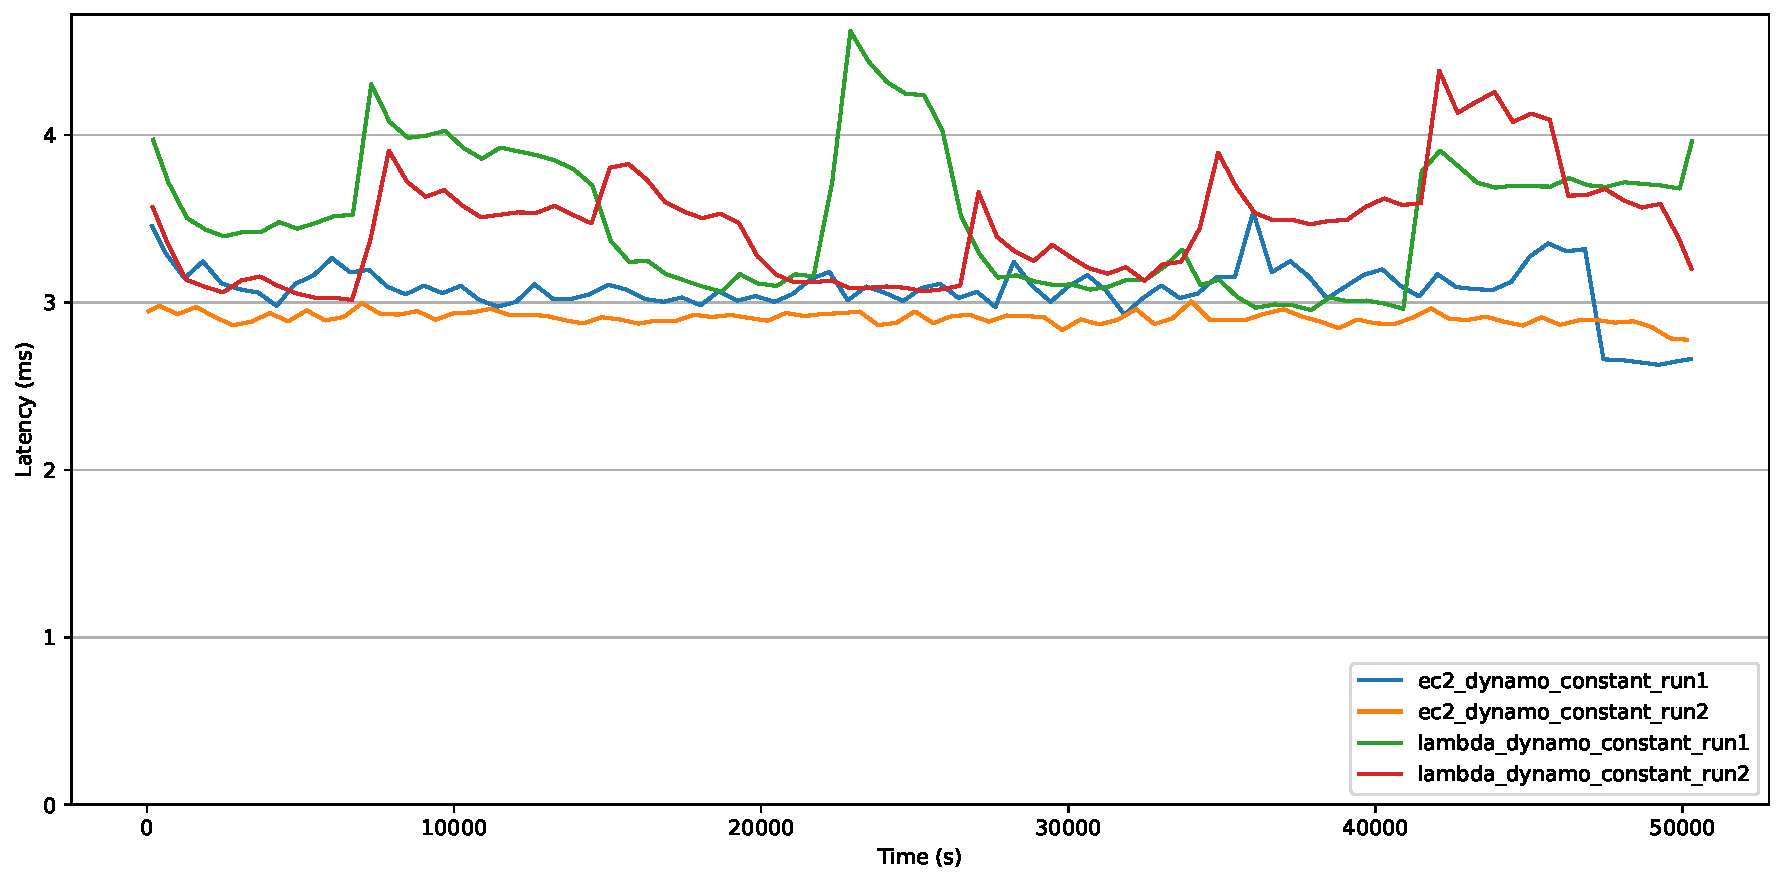
\includegraphics[width=\linewidth]{./fig/ts-dynamo-constant.pdf}
		\caption{Constant Load on DynamoDB}
		\label{fig:ts_ddb_const}
	\end{subfigure}
	\hfill
	\begin{subfigure}{0.49\linewidth}
		\centering
		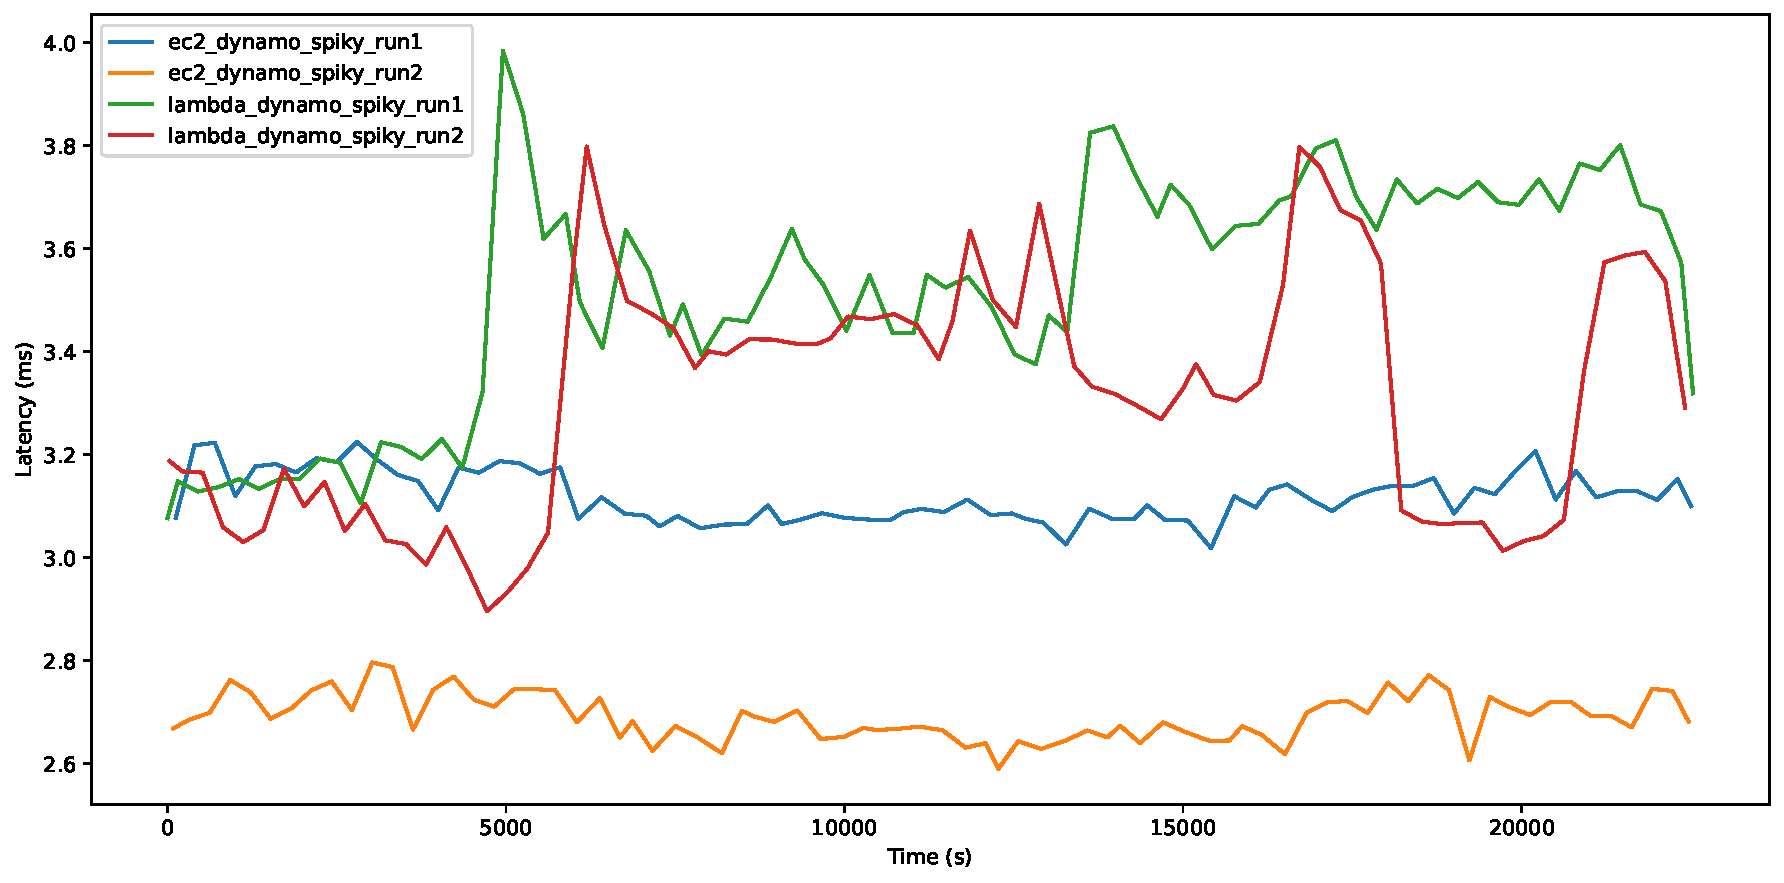
\includegraphics[width=\linewidth]{./fig/ts-dynamo-bursty.pdf}
		\caption{Bursty Load on DynamoDB}
		\label{fig:ts_ddb_bursty}
	\end{subfigure}
	\vfill
	\begin{subfigure}{0.49\linewidth}
		\centering
		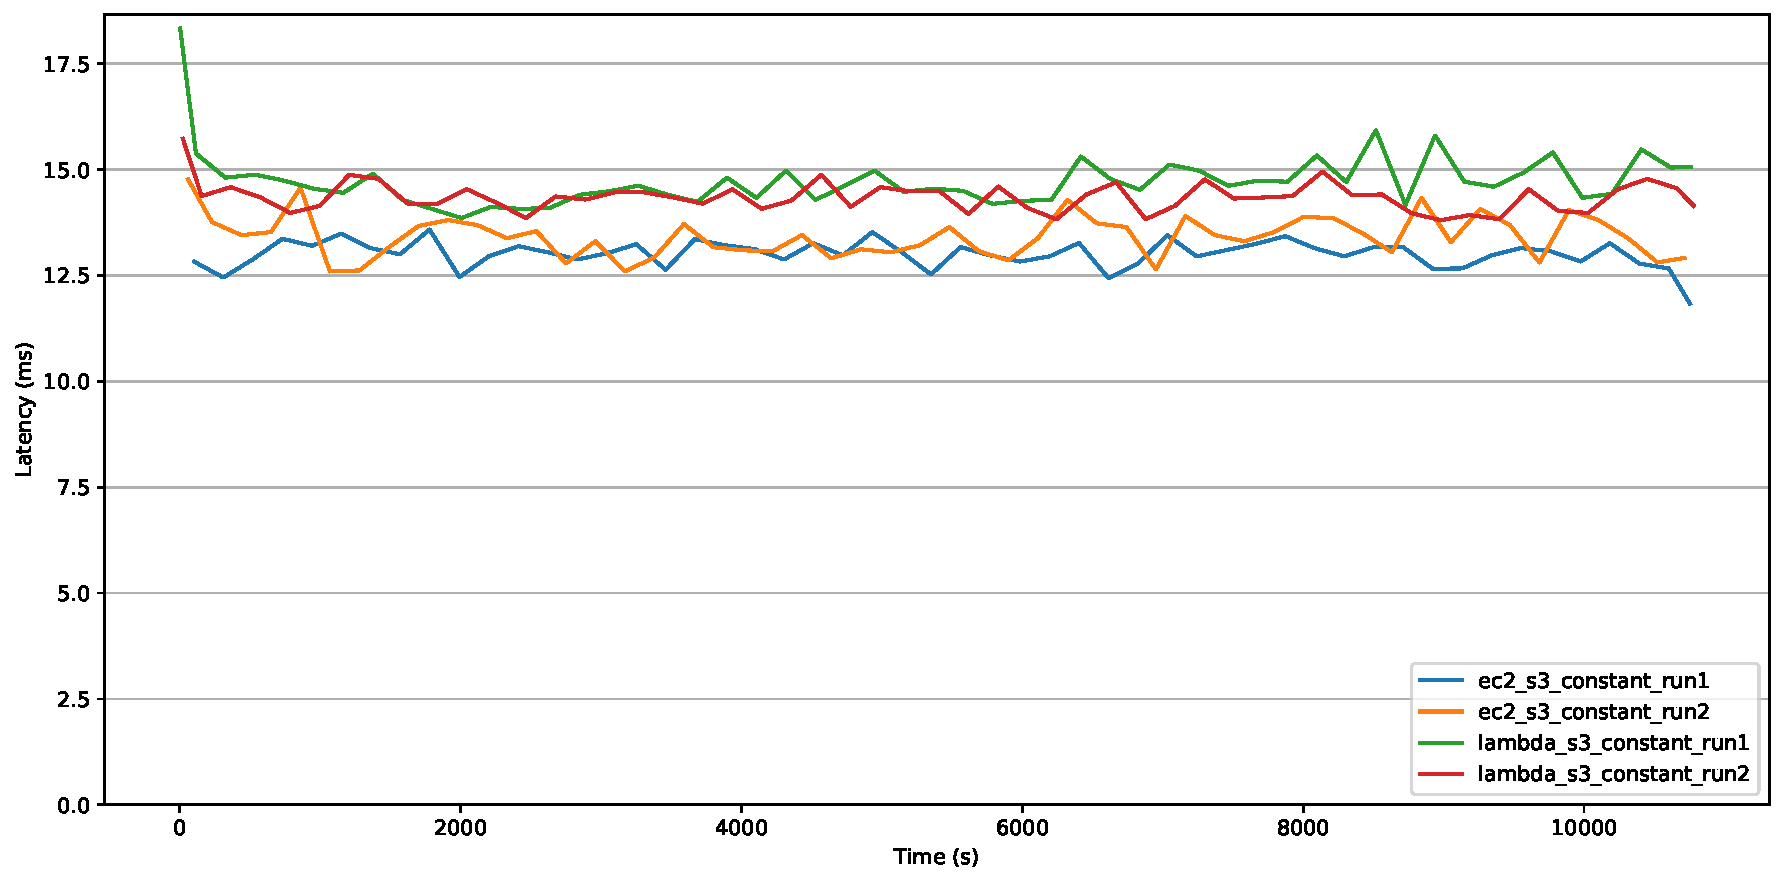
\includegraphics[width=\linewidth]{./fig/ts-s3-constant.pdf}
		\caption{Constant Load on S3}
		\label{fig:ts_s3_const}
	\end{subfigure}
	\hfill
	\begin{subfigure}{0.49\linewidth}
		\centering
		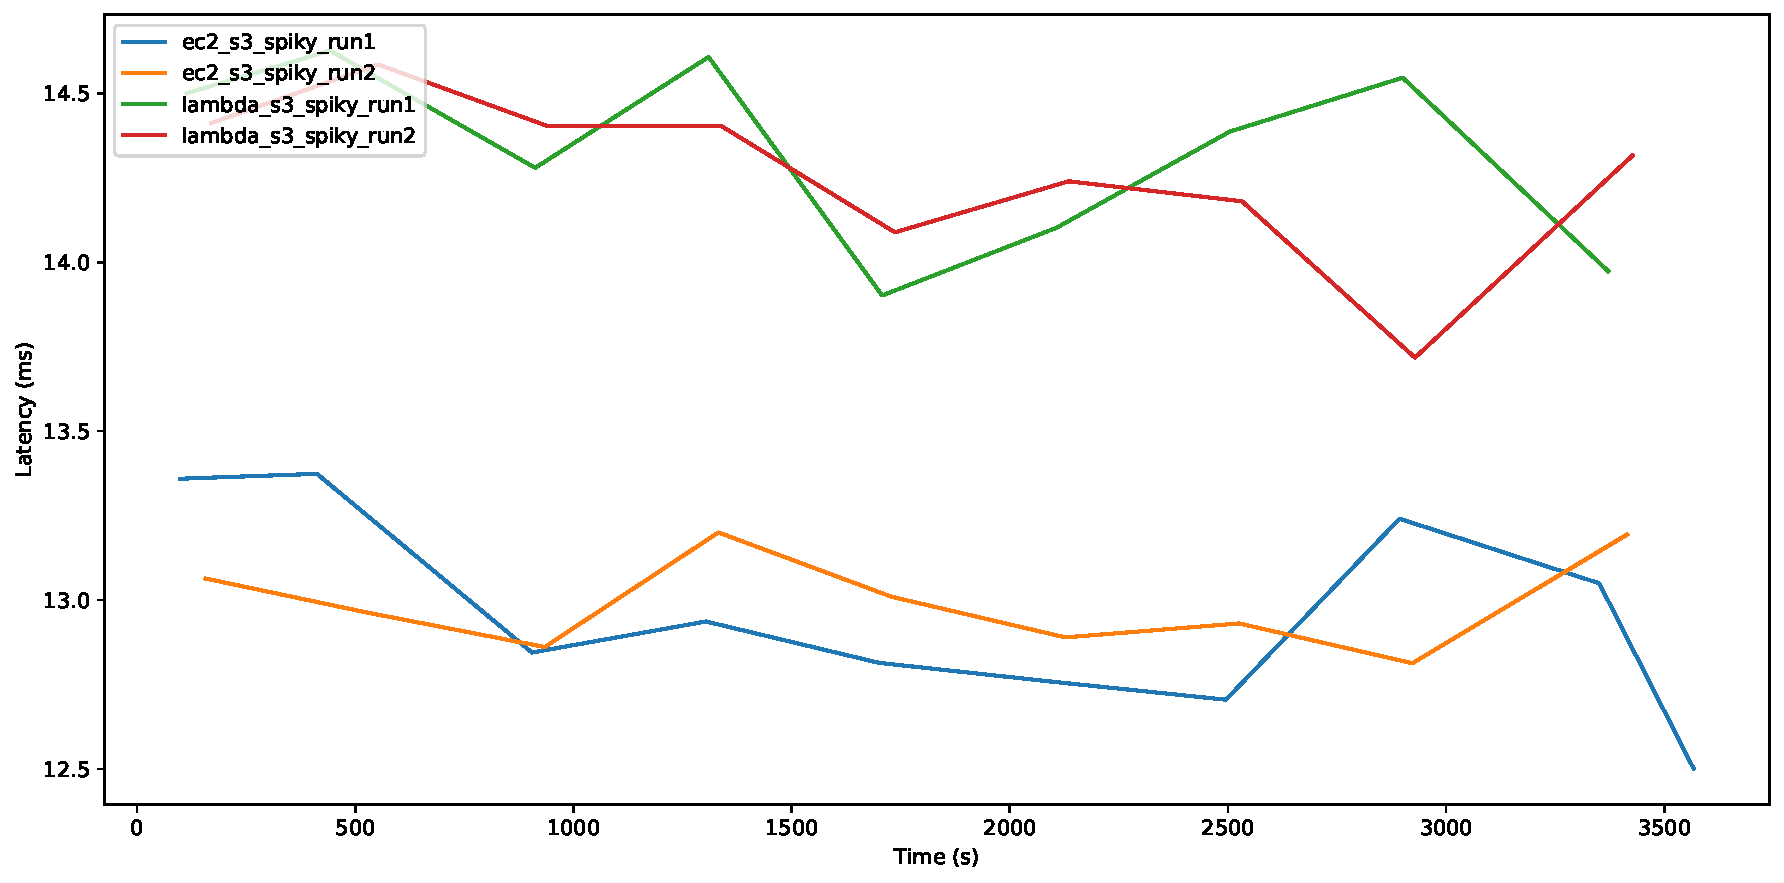
\includegraphics[width=\linewidth]{./fig/ts-s3-bursty.pdf}
		\caption{Bursty Load on S3}
		\label{fig:ts_s3_bursty}
	\end{subfigure}
	\caption{Time-Series Representation of Latency Metric}
	\label{fig:ts-plots}
\end{figure}

As observed in \cref{fig:bar-plots}, mean latencies of EC2-Pairs is less than that of Lambda-Pairs for all experiments. The absolute difference is although minimal, always less than 1.34 milliseconds. 

In \hyperref[fig:bar_s3_const]{Figure 4.1.5}, we can obeserve that EC2-S3 under constant load shows approximately 3x variance compared to EC2-S3 under bursty load in \hyperref[fig:bar_s3_bursty]{Figure 4.1.6}, which intuitively seems contradicting. Similar is observed in \cref{fig:ts-plots}, especially in \hyperref[fig:ts_rds_const]{Figure 4.2.1}, where latency with lambda suddenly rises or sinks and continues at that rate for multiple hours. Possible reason is that the underlying conditions of the cloud vary depending on day and time, leading to variations in latency performance \cite{}.

The reason behind EC2 outperforming Lambda possibly lies in the fact that, Lambdas reside inside Firecracker-VMs, which are deployed on multi-tenant EC2s. The Lambdas communicate with the host EC2s via istio-based network interface. This introduces networking overhead which might impact latency performance \cite{}.

\paragraph*{EC2-RDS vs. Lambda-RDS}

\paragraph*{EC2-DynamoDB vs. Lambda-DynamoDB}

\paragraph*{EC2-S3 vs. Lambda-S3}

\paragraph*{Outliers}
